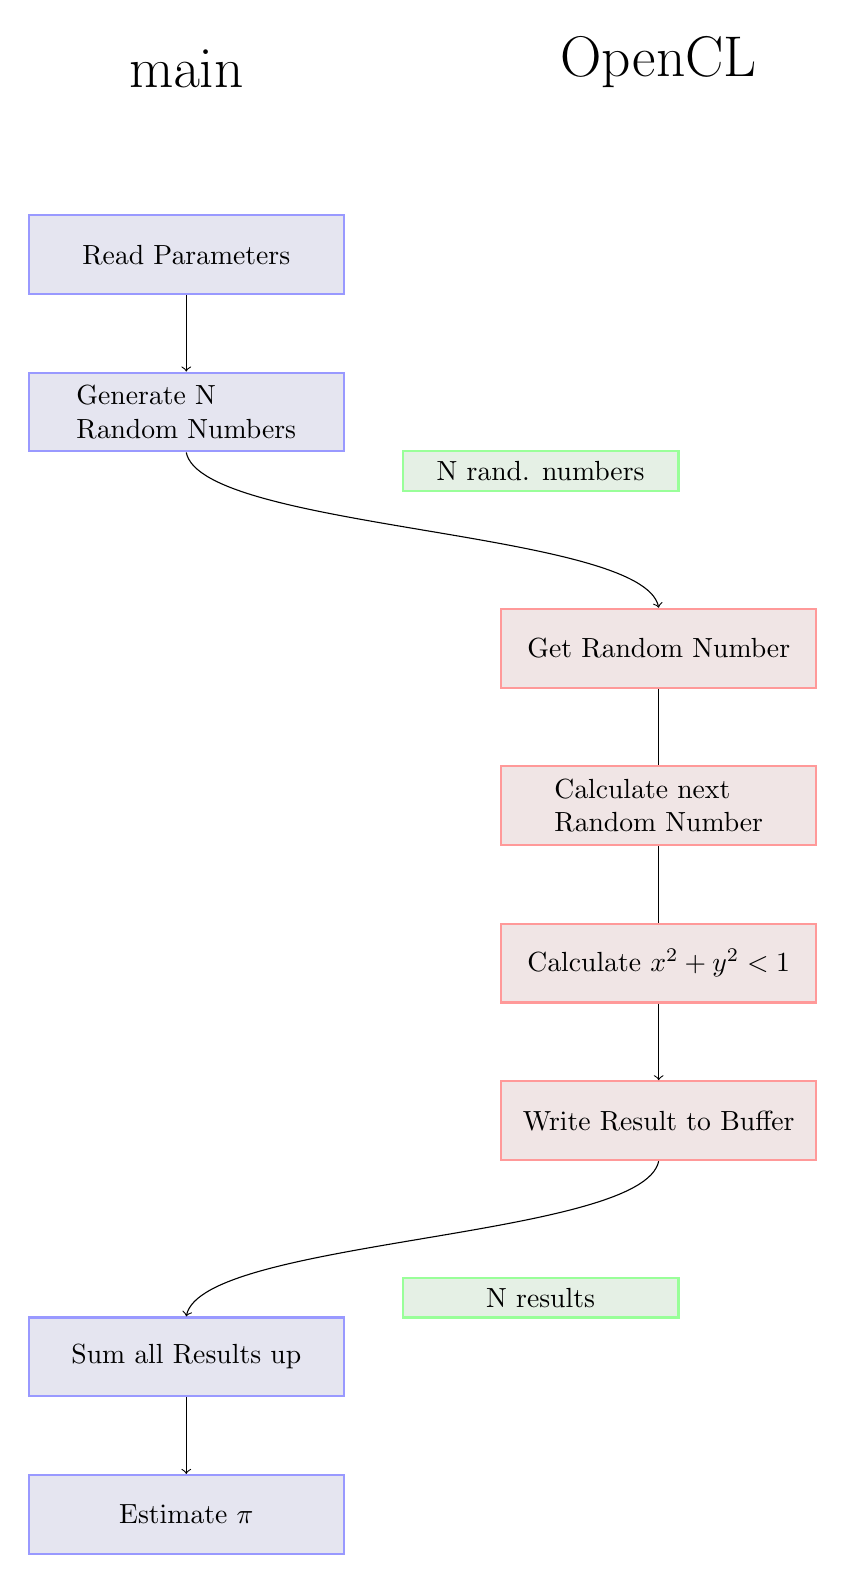
\begin{tikzpicture}[
	mainnode/.style={rectangle,draw=blue!100!black!40,fill=blue!40!black!10, thick, minimum size=1cm, minimum width=4cm,align=left},
	openclnode/.style={rectangle,draw=red!100!black!40,fill=red!40!black!10, thick, minimum size=1cm, minimum width=4cm, align=left},
	datanode/.style={rectangle,draw=green!100!black!40,fill=green!40!black!10, thick, minimum size=0.5cm, minimum width=3.5cm}
]

% Titel
\node[anchor=south,font=\huge] at (0,0) {main};
\node[anchor=south,font=\huge] at (6,0) {OpenCL};

% Ablauf
\node[mainnode] (1) at (0,-2) {Read Parameters};
\node[mainnode] (2) at (0,-4) {Generate N \\ Random Numbers};

\node[openclnode] (3) at (6,-7) {Get Random Number};
\node[openclnode] (4) at (6,-9) {Calculate next \\Random Number};
\node[openclnode] (5) at (6,-11) {Calculate $x^2+y^2 < 1$};
\node[openclnode] (6) at (6,-13) {Write Result to Buffer};

\node[mainnode] (7) at (0,-16) {Sum all Results up};
\node[mainnode] (8) at (0,-18) {Estimate $\pi$};

\draw[->] (1) -- (2);
\draw[->] (2.south) .. controls (0.2,-5.5) and (5.8,-5.5) ..  (3.north);
\draw[->] (3) -- (4) -- (5) -- (6);
\draw[->] (6.south) .. controls (5.8,-14.5) and (0.2,-14.5) .. (7.north);
\draw[->] (7) -- (8);

% Daten
\node[datanode]  at (4.5,-4.75) {N rand. numbers};
\node[datanode]  at (4.5,-15.25) {N results};

\end{tikzpicture}